This chapter presents the architecture used to enable the integration of energy storage models into a co-simulation. Section \ref{extended_co-simulation_architecture} elaborates on the existing Vessim architecture for energy storage modeling, and extends it. Afterward, Section \ref{energy_storage_interface} describes the interface this approach uses for the implementation of battery pack models at multiple levels of complexity, whereas Section \ref{energy_management_policies} discusses, how policies are defined, which are used to balance the energy within a microgrid simulation at every time-step, and are necessary to perform the required energy management in the co-simulator.

\section{Extended Co-Simulation Architecture}
The structure of a co-simulated microgrid, according to Wiesner et al. \cite{vessim}, was already presented in Section \ref{vessim_architecture}. It is now being refined to include an energy storage interface, energy management policies, and new connections between the storage simulation unit and the controller simulators. Figure \ref{fig:co_simulation_architecture} depicts the resulting architecture.

\label{extended_co-simulation_architecture}
\begin{figure}[t]
    \centering
    \includegraphics[width=\linewidth]{thesis/Images/Co_Simulation_architecture.pdf}
    \caption{Refined Co-Simulation structure with the proposed energy storage interface.}
    \label{fig:co_simulation_architecture}
\end{figure}

The defined \textbf{Storage} and \textbf{MicrogridPolicy} objects, detailed in the following sections, are included in the Vessim storage simulator, which is the last simulator to step, modeling the progression of time between time-steps. As mentioned, at every time-step $t$, the storage simulation unit receives $\Delta p_t$ through the Mosaik Scheduler (see Section \ref{mosaik_framework}). This $\Delta p_t$ marks the power delta of the energy producers and consumers, as obtained by the grid simulation unit utilizing a power flow analysis, and, along with the duration of the time-step $d$, is passed to the \textbf{MicrogridPolicy} object. The value of $d$ is known because the storage simulation unit is continuous-time based while implementing the Mosaik API, and therefore includes a step-size. Using these parameters, the policy is applied as explained in Section \ref{energy_management_policies}, utilizing the energy storage interface defined in Section \ref{energy_storage_interface}.

The return value of that function call indicates the energy $e_t$ taken from or fed into the utility grid during the last time-step $t$. This value is passed to the controllers using the Mosaik Scheduler, together with the updated state of the storage $state_{t+1}^s$ (defined in Section \ref{energy_storage_interface}). That way, the architecture provides the controllers, and thereby also carbon-aware applications, \textit{visibility} over the power system, which is one of the key ideas behind the Vessim framework. Because the storage simulation unit is stepped after the controllers, the message passing between the simulation units is cyclic, meaning that the controllers receive the energy delta of the previous time-step $t-1$, and the storage state at the beginning of the time-step $t$.

In addition to this provision of \textit{visibility}, another requirement of the Vessim architecture is to enable \textit{control} over the simulated microgrid. In terms of the energy management and the energy storage, the topics that this thesis focuses on, \textit{control} means that the controllers can tweak the configuration of the energy storage system during simulation runtime, as the Vessim paper \cite{vessim} already describes how applications can interact with the controllers via an API through Software-in-the-loop simulation. This is achieved again using the message passing of the Mosaik Scheduler, as the  controllers can send a collection of key-value pairs to the storage simulation unit, where they are handled so that relevant functions for the updating of parameters are called on the \textbf{MicrogridPolicy} or \textbf{Storage} objects. Thus, the responsibility for defining the parameters that can be updated during runtime lies with the developer of the models and policies.

\section{Energy Storage Interface}
\label{energy_storage_interface}
One of the main goals of this work is to describe a common interface for energy storage models to be used inside a microgrid co-simulation. This interface should be adaptable enough so that the complexity range of these models is not too limited, but has to be simple enough to allow a clear co-simulation architecture that still separates power consumption and power generation from the process of storing energy.

Due to the underlying Vessim architecture \cite{vessim}, which conducts power flow analysis, the main input to the battery models is power instead of current, which would be the common input to complex models like the SPM (see Section \ref{single_particle_models}). Additionally, a management system is modeled as part of the battery, similarly to what is described by Kazhamiaka et al. \cite{kazhamiaka2018pimodel} in their paper discussing the PI-model as described in Section \ref{c_l_c_model}. The reason behind that is to not allow simulated batteries to be used in ways that would be prevented by a BMS (see Section \ref{battery_management_systems}) like over- or undercharging, and to again provide the necessary \textit{visibility} over the storage.

In the proposed design, the \textbf{Storage} provides the abstract interface for a battery system, which allows for charging and discharging operations, and contains the monitoring and control functionality of a BMS. The primary function of the interface is to handle the energy flow into and from the battery, which is facilitated through an update method, receiving the power to be (dis-)charged $p_s$ as well as the (dis-)charging duration $d_s$. The \textbf{Storage} adjusts its internal state based on these parameters, whereas the included BMS watches that the defined limits of the battery are respected. In the end, the function returns the total amount of energy $e_s$ that has been stored or discharged during this timeframe. For instance, if the battery was requested to charge at $p_s = 20W$ for $d_s = 10s$, but the BMS limits the charging to $15W$, the return value would be $e_s = 15W \cdot 10s = 150Ws$.

In addition to this basic charging and discharging, a \textbf{Storage} implementing the energy storage interface has to include functionality to allow for monitoring of the battery's internal state. As discussed in Section \ref{battery_management_systems}, the SoC is the key metric when it comes to determining the energy level of a battery, and therefore, there has to be a way for the BMS to give an estimation that can be used for energy management in the microgrid. For other important internal parameters that depend on the type of battery, the \textbf{Storage} can also define a custom state $state^{s}$ that can be used for providing visibility over the battery system. The state is transmitted to the controllers via the Mosaik scheduler as described in Section \ref{extended_co-simulation_architecture}.

\section{Energy Management Policies}
\label{energy_management_policies}
\begin{figure}[t]
    \centering
    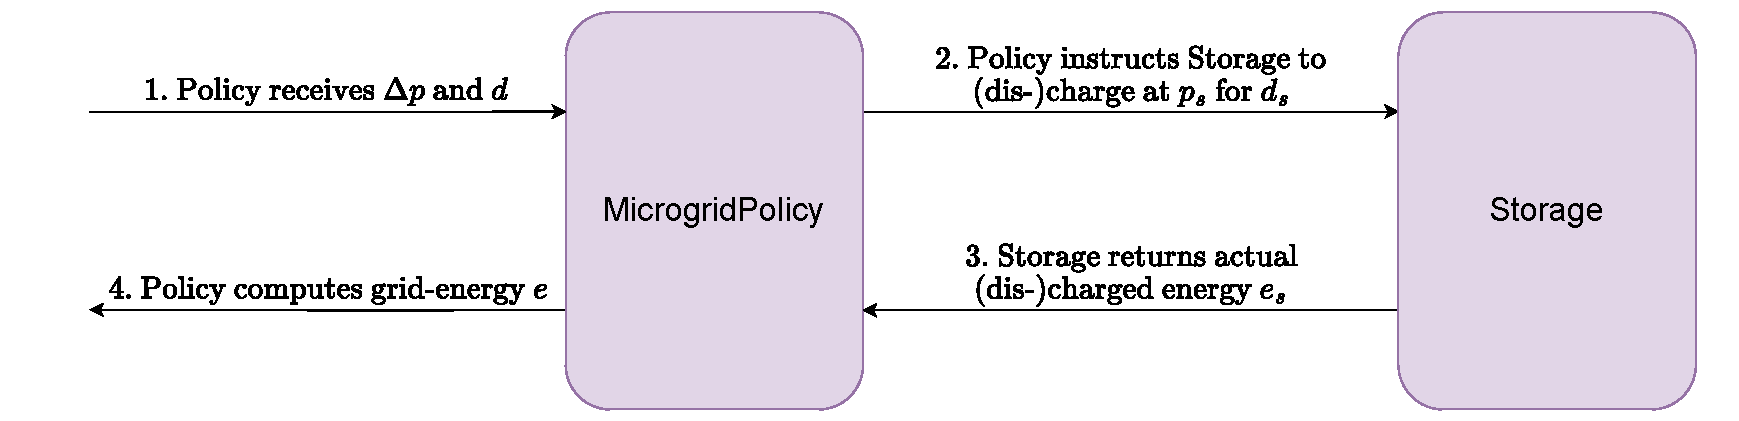
\includegraphics[width=\linewidth]{thesis/Images/Microgrid_Policy.pdf}
    \caption{Interactions between the \textbf{MicrogridPolicy} and the \textbf{Storage}.}
    \label{fig:microgrid_policy}
\end{figure}
In the context of microgrid co-simulation, energy management is a critical part, as it has to be defined, how the microgrid responds to specific power deltas, which refer to the variations in power supply and demand. For this purpose, the approach allows for a user-defined \textbf{MicrogridPolicy}, which provides a structured way to deal with these power fluctuations, whereas the management includes interactions with the public grid and present energy storage systems as well as curtailment.

The policy lets users define custom rules and strategies that balance the power delta of the microgrid's generators and consumers at every time-step. In case of excess power during the time-step, energy has to be stored, fed back to the utility grid, or curtailed, while a lack of power has to be leveled using either grid energy or the energy received by discharging the energy storage. These rules are applied at every time-step based on the current power delta, the duration that the delta is valid for, and also the battery's SoC as computed by the \textbf{Storage}.

When the \textbf{MicrogridPolicy} is applied, it receives the current power delta $\Delta p$ (see section \ref{vessim_architecture}) and the time $d$ that passed since the last time-step. With the defined rules, the policy then decides, what portion of the power delta is to be balanced by charging or discharging the \textbf{Storage} that the policy can access. It then instructs the \textbf{Storage} to (dis-)charge with a power $p_s$ for a specified duration $d_s$ that should be equal to, or, in special cases, less than $d$.

As discussed in section \ref{energy_storage_interface}, the \textbf{Storage} returns the actual energy $e_s$ that could be charged or discharged given these inputs when it is updated. The policy finally uses that to compute the amount of energy $e$ that the microgrid had to draw or that the microgrid could feed into the public utility grid during the time-step. The mentioned interactions between the \textbf{MicrogridPolicy} and the \textbf{Storage} are also depicted in Figure \ref{fig:microgrid_policy}. In the most basic case, where no energy is curtailed, and the microgrid can exchange energy with the public grid at all times, the grid energy can be computed using the formula $e = \Delta p \cdot d - e_s$, where $\Delta p \cdot d$ marks the total energy surplus or deficit of the microgrid since the last time-step. If $e$ was greater than zero, there was energy fed to the grid, and in the case of $e$ being less than zero, energy had to be drawn from the grid.

The \textbf{MicrogridPolicy} separates itself from the BMS of the energy storage in the way that it can also handle energy flow from or to the public grid, and can be, for instance, used to model the operating mode (grid-connected or islanded as defined in section \ref{microgrids}) of the microgrid. Because the \textbf{MicrogridPolicy} only has access to the abstract energy storage interface, it is also more general, as it does not depend on the battery model in comparison to the BMS.